%%---------------------------------------------------------------------
%	Preamble
%	AMS gruppe 12
%	AMS F18
%---------------------------------------------------------------------
\documentclass[12pt,fleqn,a4paper]{article}
\usepackage[utf8]{inputenc}
\usepackage[danish]{babel}
\usepackage[top=2.5cm, left=2cm, right=2cm, bottom=2.5cm]{geometry}
\usepackage{graphicx}
\usepackage[bottom]{footmisc}
\usepackage{framed}
\usepackage{caption}
\usepackage{float}
\usepackage{mdframed}
\usepackage{listings}
\usepackage{color}
\usepackage[T1]{fontenc}
\usepackage{amsmath,amsfonts,amsthm} % Math packages
\usepackage{array}
\usepackage{wrapfig}
\usepackage{multirow}
\usepackage{tabu}
\usepackage{longtable}
\usepackage{lastpage}
\usepackage{fancyhdr}
\usepackage[compact]{titlesec}
\usepackage[table,xcdraw]{xcolor}
\usepackage{arydshln}
\usepackage[isbn,issn,url]{dk-bib}
\usepackage[toc,page]{appendix}
\usepackage{url}
\def\UrlBreaks{\do\/\do-}

\definecolor{mygreen}{RGB}{28,172,0} % color values Red, Green, Blue
\definecolor{mylilas}{RGB}{170,55,241}
\renewcommand{\lstlistingname}{Kodeudsnit}
\tabulinesep=3mm

\setcounter{secnumdepth}{2}
\setcounter{tocdepth}{2}

\setlength{\parindent}{0mm} %intet indryk
\setlength{\parskip}{3mm} 	%linjeskift v. afsnit

% Ændring af enumerize og itemize 
\usepackage{enumitem} % @http://ctan.org/pkg/enumitem
\setlist[itemize]{topsep=0pt, itemsep=0.5pt}
\setlist[enumerate]{topsep=0pt, itemsep=0.5pt}

%afstand omkring sections
\titlespacing{\section}{0pt}{5mm}{0pt}
\titlespacing{\subsection}{0pt}{2mm}{0pt}
\titlespacing{\subsubsection}{0pt}{2mm}{0pt}

\usepackage{arydshln}
%aryd
\setlength\dashlinedash{3pt}
\setlength\dashlinegap{4pt}

\lstset{language=C++,
	breaklines=true,
	keywordstyle=\color{blue},
	stringstyle=\color{red},
	commentstyle=\color{mygreen},
	morecomment=[l][\color{magenta}]{\#}
}

%header & footer
\makeatletter
\pagestyle{fancy}
\fancypagestyle{plain}{}
\renewcommand{\chaptermark}[1]{\markboth{#1}{}}
\setlength{\headheight}{35pt}
\fancyfoot{} % clear all fields
\fancyfoot[R]{Side \thepage\ af \pageref{LastPage}}
\fancyhead{} % clear all fields
\fancyhead[L]{
\includegraphics[clip, trim = 0 0 240pt 0, height=30pt]{Figur/IHA_AU_logo.png}}
\fancyhead[R]{Forår 2018}
\fancyhead[C]{Anvendte Microcontroller Systemer}
\renewcommand{\headrulewidth}{0pt}

\def\thickhrulefill{\leavevmode \leaders \hrule height 1.2ex \hfill \kern \z@}
\def\@makechapterhead#1{
  \vspace*{10\p@}%
  {\parindent \z@ \centering \reset@font
        \thickhrulefill\quad 
        \scshape\bfseries\textit{\@chapapp{}  \thechapter}  
        \quad \thickhrulefill
        \par\nobreak
        \vspace*{10\p@}%
        \interlinepenalty\@M
        \hrule
        \vspace*{10\p@}%
        \Huge \bfseries #1 \par\nobreak
        \par
        \vspace*{10\p@}%
        \hrule
        \vskip 40\p@
  }}

\usepackage{tcolorbox}
\definecolor{mycolor}{rgb}{0.122, 0.435, 0.698}% Rule colour
\makeatletter
\newcommand{\mybox}[1]{%
	\setbox0=\hbox{#1}%
	\setlength{\@tempdima}{\dimexpr\wd0+13pt}%
	\begin{tcolorbox}[colframe=mycolor,boxrule=0.5pt,arc=4pt,
		left=6pt,right=6pt,top=6pt,bottom=6pt,boxsep=0pt]
		#1
	\end{tcolorbox}
}
\makeatother

\graphicspath{ {Figur/} }


%Se Kodeudsnit \ref{lstlisting:generel_kode}

%\captionof{lstlisting}{Generelle egenskaber for koden til fremstilling af diverse figure i matlab} 
%\label{lstlisting:generel_kode}
%\vspace{5mm} %5mm vertical space
%
%\subsection{Kode til lyd i forhold til tiden}
%\begin{framed}
%\begin{center}
%\begin{lstlisting}
%figure('name','trafikstoejen i fuld laengde'); clf
%subplot(211);
%plot(t,s_sound_left)
%xlabel('Tid (sek)')
%ylabel('Signalstyrke')
%title('Trafikstoej set i forhold til tiden')
%grid on
%hold on
%\end{lstlisting}
%\end{center}
%\end{framed}




%\begin{document}

\section{Købt hardware}
Robottens chassis og mekaniske dele er købt som et samlesæt. 
Motorerne er DC-motorer med gearing, og aksler til montering af hjul.
Billeder af købt hardware kan findes i bilag \ref{appendix:BilagKoebtHardware}.
Den dobbelte H-bro, der fulgte med robotten, er af modellen \textit{L298N}, og er integreret på et print med egen strømregulering og sikkerhedsafkobling. 
Printet har terminaler til forsyningsspænding, styring samt forskellige tilbagekoblinger.
\newpage
\subsection{Enhedstest}
Den købte hardware skal kunne opfylde følgende krav:
\begin{itemize}
\item Motorerne skal kunne køre ved en tilsluttet spænding mellem $9V - 12V$
\item Robotten skal kunne dreje om egen akse
\item Bilen skal have dimensioner på mindre end 40x40x40 cm - som beskrevet i kravspecifikationen. 
\end{itemize}

Test af disse krav kan findes i bilag \ref{appendix:BilagTestKoebtHardware}.

Ud fra testene kan det konkluderes, at den købte hardware kan bruges til projektet. Dog blev det ved testen også opdaget, at motorerne kører forskelligt i en sådan grad, at regulering er nødvendigt for, at robotten vil kunne køre lige.

\section{Spændingsforsyning}
Robotten skal forsynes med strøm fra et batteri. Ud fra de ikke-funktionelle krav, er der valgt et batteri med en DC-spænding målt til ca. $10.5 V$ ved fuld opladning.

For at forsyne PSoC'en, Pi'en og sensorerne med $5 V$, bruges en linear regulator af typen \textit{LM350T} til at regulere batterispændingen ned til ca. 5V - som specificeret i signaltabellen i bilag \ref{appendix:signalbeskrivelse}.

\subsection{Enhedstest}
For at teste, at spændingsforsyningen virker som ønsket, laves en test, hvor det sikres, at regulatoren kan levere $5 V$ med en forsyningsspænding fra $ 9-12 V $, som specificeret i signaltabellen i bilag \ref{appendix:signalbeskrivelse}. 
Testen kan findes i \ref{appendix:Bilag_enhedstest_spaendingsforsyning}.

Efter testen er det konkluderet, at spændingsforsyningen kan bruges til projektet, da den er i stand til at levere ca. 5V i intervallet $12 V$ til ca. $7 V$.

Efter testene blev der målt, hvor meget strøm, der trækkes igennem transistoren. Her blev der målt, at der trækkes  ca. $500 mA$ under brug - hovedsagligt fra Pi'en.
Dette resulterer i, at der bliver afsat en betragtelig effekt i spændingsregulatoren, så den bliver varm. 
For at kompensere for temperaturændringen er der påsat en køleplade. 
IHA's størst tilgængelige køleplade kan holde transistoren på ca. $70^{\circ}C$, hvilket ikke er særligt langt under den opgivede maksimale operationstemperatur på $125^{\circ}C$. \\
For at forlænge levetiden på produktet, kunne der enten vælges en større køleprofil eller en anden spændingsregulator, med et større safe operating area.
\newpage
\section{Motorkontrolenhed}
I dette afsnit beskrives enheden, som bruges til styring af robottens motorer. 

For at forbedre oplevelsen for brugeren, reguleres motorerne på robotten til at køre lige hurtigt, så robotten kører ligeud.
Derudover fremgår det også af kravene, at motorstyringen skal være i stand til at informere systemet, om robotten er i bevægelse eller ej. \\
Til at styre robotten benyttes en \textit{PSoC 5LP}. 
Denne er valgt, fordi gruppen har erfaring med at bruge microcontrolleren, og den er i stand til at udføre alt ønsket funktionalitet.
 

\subsection{Motorkontrol}
Bilens fire motorer styres i par af to, så bilen drejer ved skridstyring. 
Hvert sæt motorer er tilkoblet én H-bro, der styres af PSoC'en. 
Topdesignet til motorstyringsmodulet ses på Figur \ref{fig:top_styring}.

%billlede af topdesign.
\begin{figure}[H] 
\centering
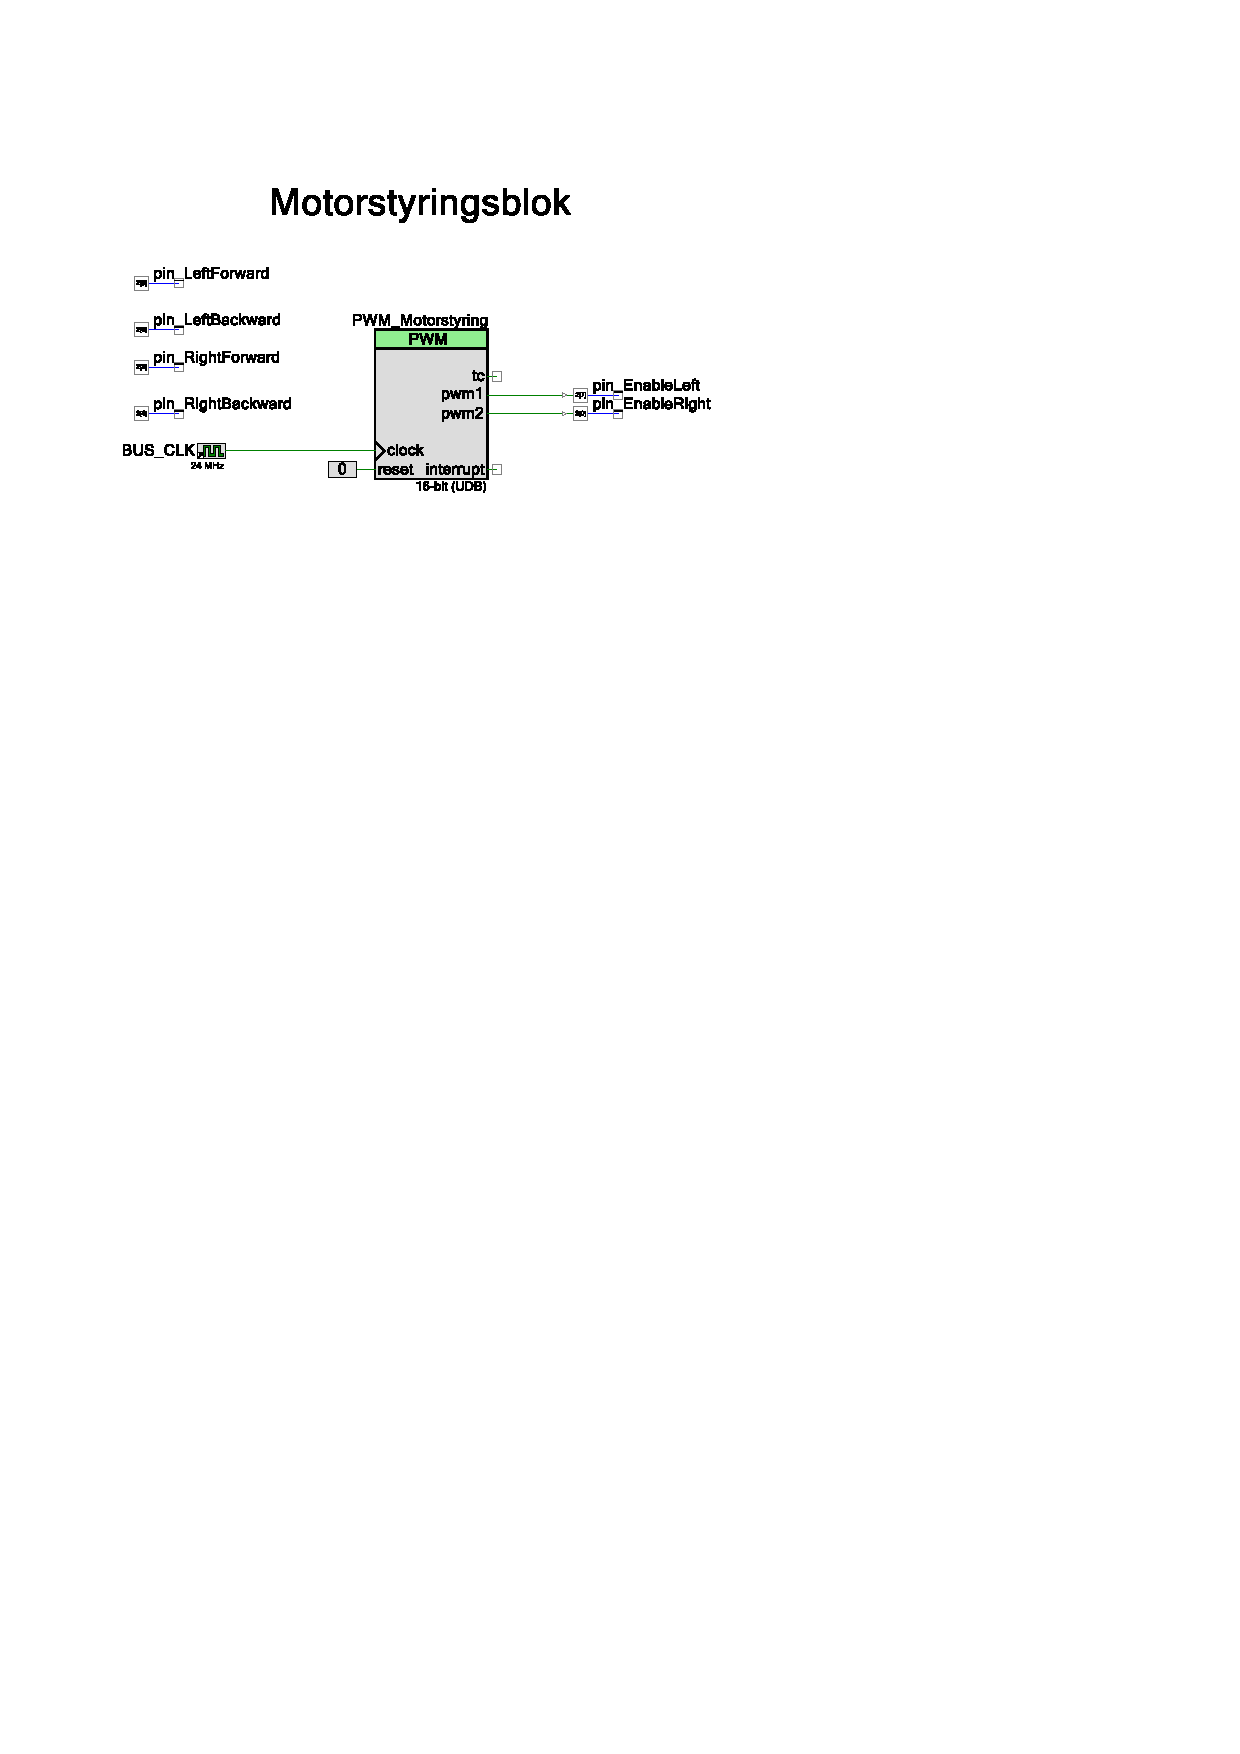
\includegraphics[clip, trim = 2cm 21.35cm 8cm 4cm , width = 0.7\textwidth]{top_styring.pdf}
\caption{Topdesign af Motorkontrol-blokken, fra PSoC Creator}
\label{fig:top_styring}
\end{figure}

PSoC'en er tilsluttet h-broen således, at to GPIO-pins bruges til at styre motorenes retning, og en tredje GPIO-pin styrer hastigheden med pulsbreddemodulation.

PWM-blokken har en opløsning på 16 bit. 
Den høje opløsning er valgt, fordi motorernes hastighed ændres markant ved relativt små ændringer i duty-cyclen - dette bliver relevant ved motorreguleringen. \\
PWM-signalets grundfrekvens er valgt til $19 kHz$, altså udenfor det hørbare spektrum for et voksent menneske. 

Motorerne styres med funktionen \textit{ControlMotors()}, der ændrer robottens retning efter input fra Kontrolenheden. 
For at gøre robotten lettere at styre, er drejehastigheden sat til at være lavere end kørehastigheden. 

\subsubsection{Enhedstest}
For at teste, at motorkontrollen gør som beskrevet, analyseres signalerne med et oscilloskop. 
Testen kan ses på bilag \ref{appendix:BilagPSoCEnhedstests}.

Ud fra testen kan det konkluderes, at motorkontrollen virker som ønsket.

\subsection{Regulering}
Motorreguleringsblokken har til ansvar at sikre, at begge hjulpar kører lige hurtigt. 
For at sikre dette, skal der være tilbagekobling fra motorerne. \\
Til at implementere tilbagekoblingen stod valget mellem at bruge optiske sensorer til at måle omdrejningstallet eller at måle strømmen gennem H-broens to current sense terminaler.
Tilbagekoblingen er implementeret med optiske sensorer, da strømmåling har følgende ulemper:

\begin{itemize}
	\item Måleusikkerhed ved PSoC'ens ADC
	\item Signalet ville i mindre grad være immunt overfor støj, hvilket kunne være et problem, da robottens motorer støjer betragteligt
	\item Strømmen gennem motorerne er ikke nødvendigvis proportionel med robottens hastighed
\end{itemize}

Ved at vælge de optiske sensorer, undgås ovenstående ulemper. 
Derudover kan de også bruges til at måle bilens hastighed, hvis dette ønskes implementeret. 
Ulempen ved de optiske sensorer er, at det kræver flere komponenter at implementere, men det er blevet vurderet, at fordelene gør op for denne ulempe.

De to optiske sensorer, der bruges, er af typen \textit{TCST 2103}. 
Sensorerne består af en infrarød LED og en fototransistor. På figur \ref{fig:koncept_optisksensor} kan en illustration af sensorernes virkemåde ses.

\begin{figure}[H] %ET BILLEDE AF FARTSENSOR
\centering
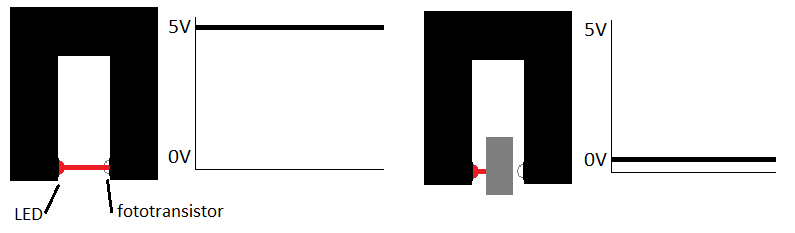
\includegraphics[clip, trim = 0cm 0cm 0cm 0cm , width = 0.8\textwidth]{koncepttegning_regulering.png}
\caption{Koncepttegning af optisk sensor}
\label{fig:koncept_optisksensor}
\end{figure}

Det ses på figuren, at når lyset fra LED'en opfanget af sensoren, så trækkes outputtet til $5 V$, og når lyset brydes trækkes outputtet lavt til stel. 

De optiske sensorer tæller omdrejnigner på to tandhjul monteret på indersiden af begge forhjul. 
Opstillingen vises på figur \ref{fig:motor_feedback}.

\begin{figure}[H] %ET BILLEDE AF FARTSENSOR
\centering
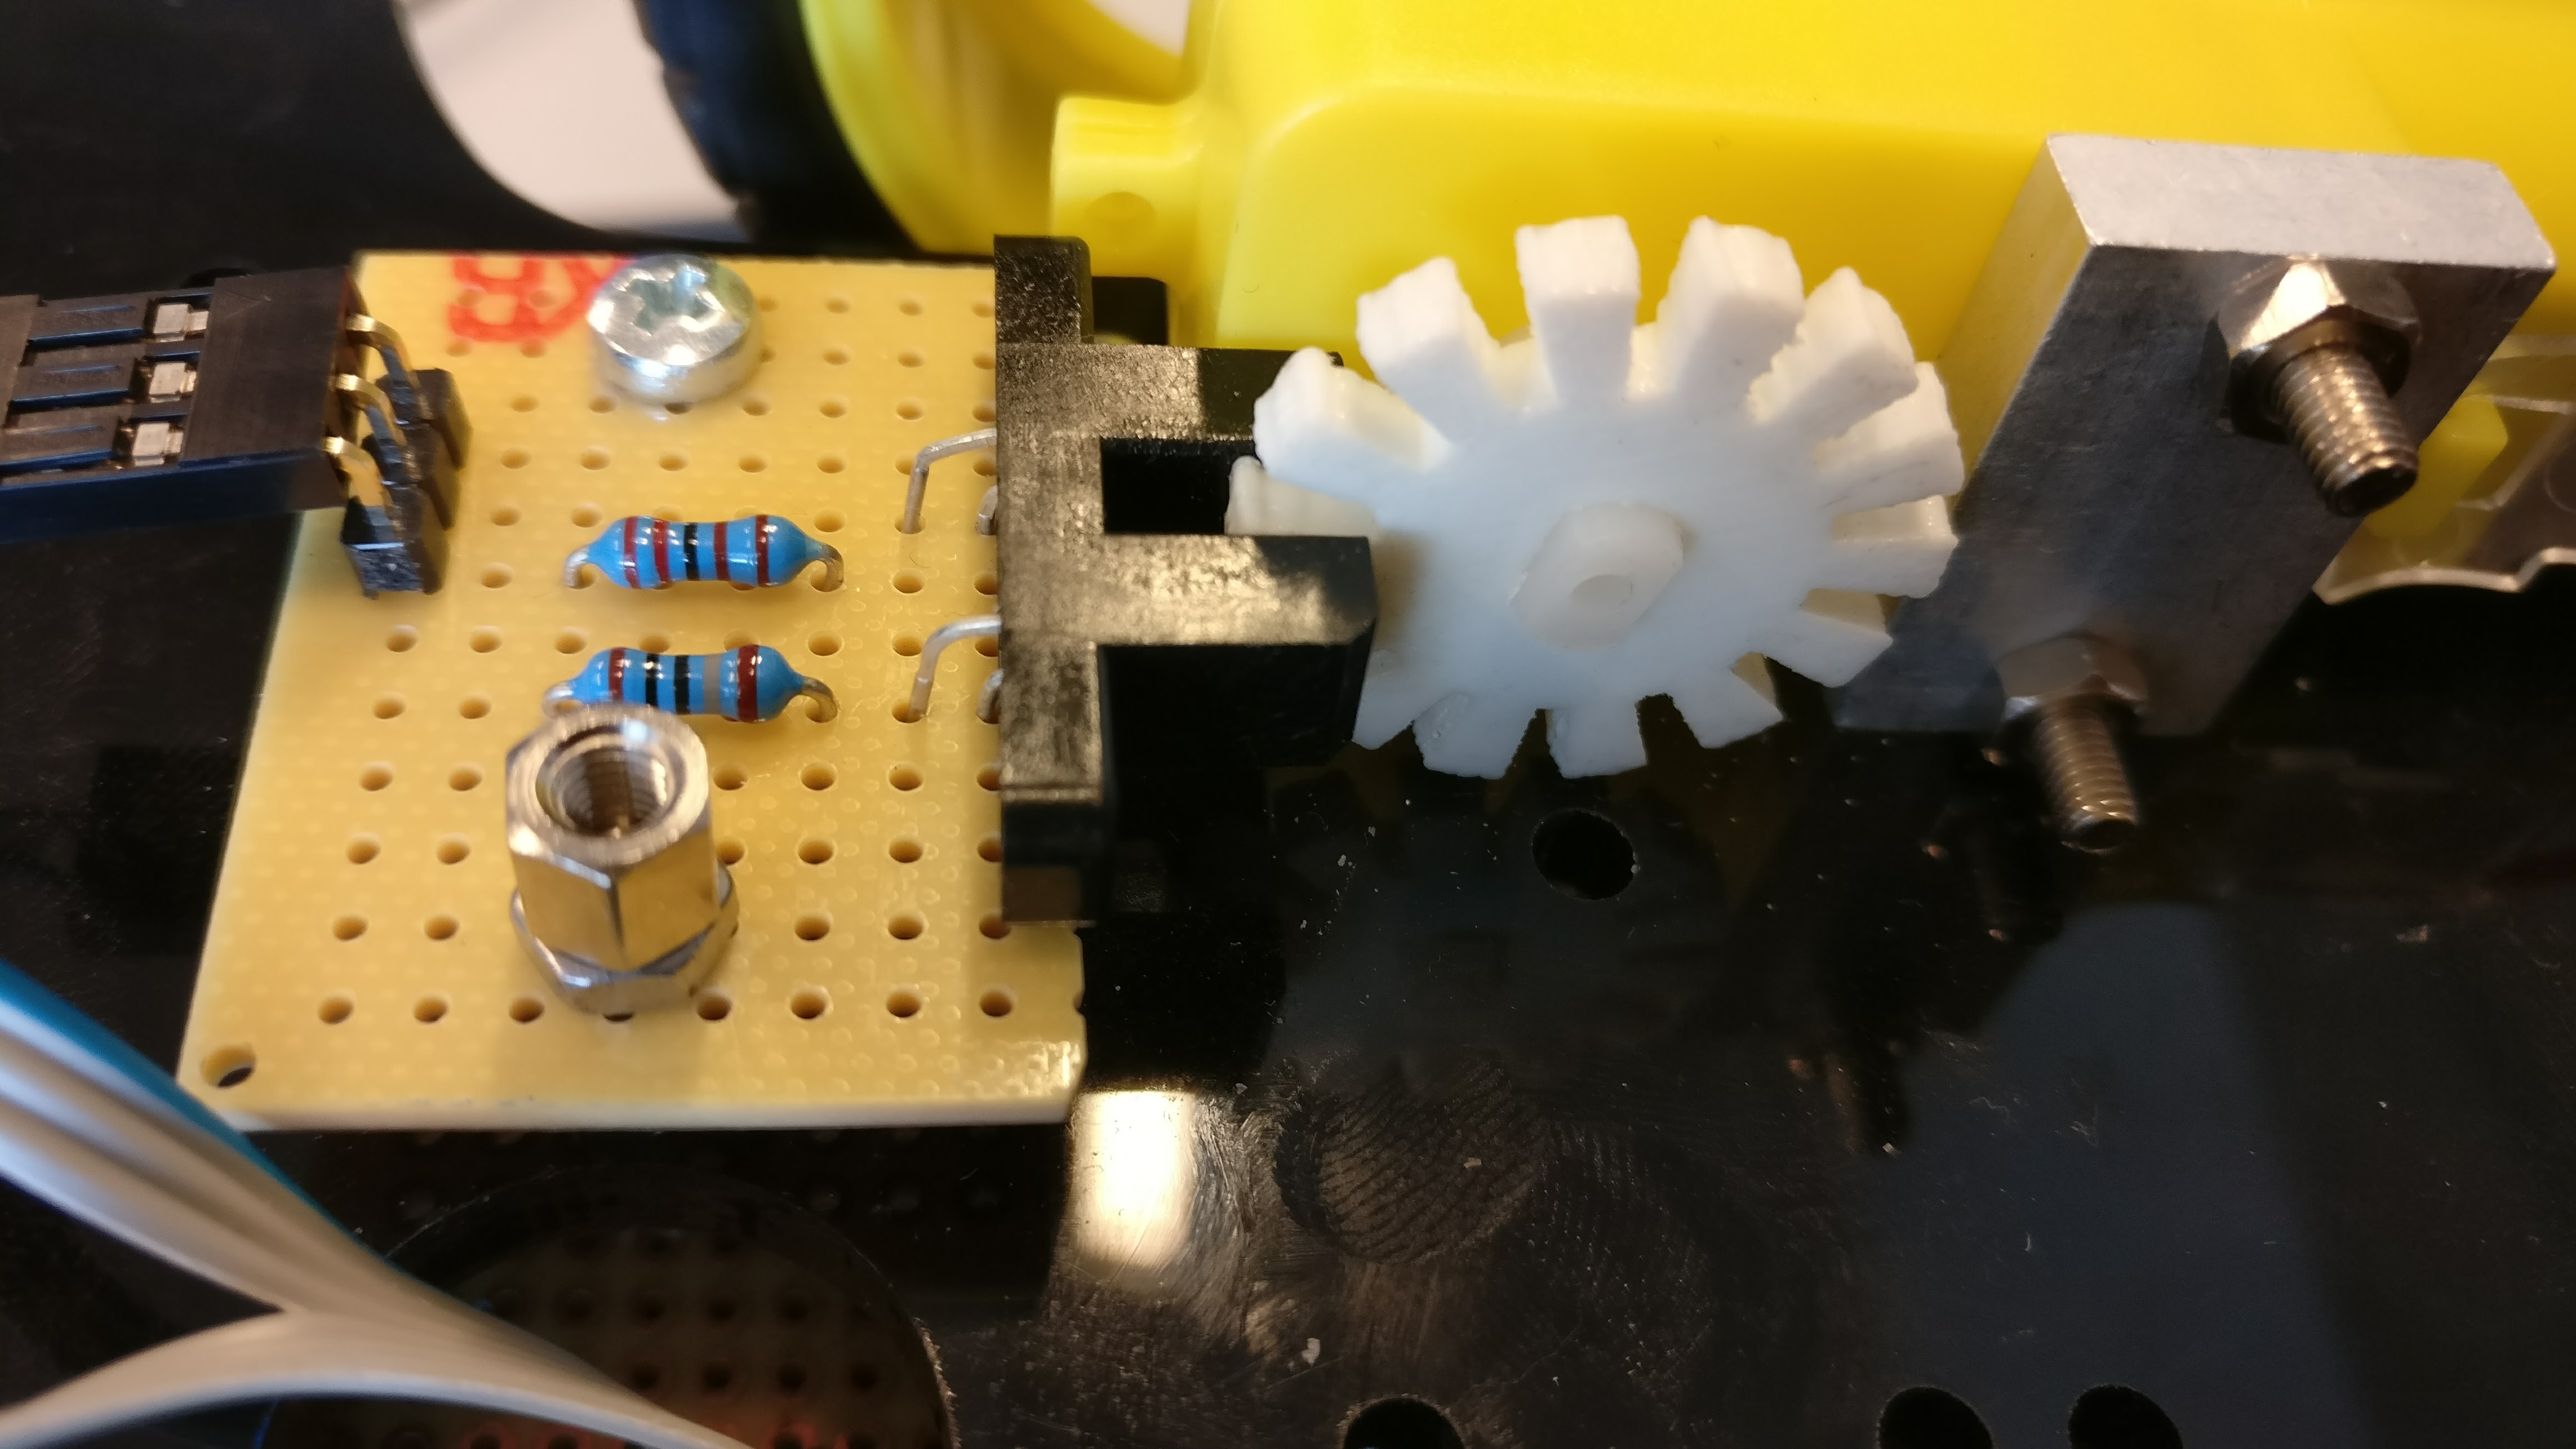
\includegraphics[clip, trim = 0cm 15cm 20cm 0cm , width = 0.5\textwidth]{Motor_Feedback.jpg}
\caption{Billede af omdrejningstæller, monteret på motor}
\label{fig:motor_feedback}
\end{figure}

Når tandhjulet kører genereres et firkantsignal, med en frekvens proportional med hjulets omdrejningshastighed. 
Hjulenes omkreds er målt til ca. $22 cm$. 
Derudfra findes robottens hastighed ved:
\begin{equation}\label{eq1}
v(f)= 22cm \cdot \frac{f}{n}\,
\end{equation}
hvor $f$ er frekvensen i $Hz$ og $n$ er antal spalter i tandhjulet. 

Omdrejningstælleren er koblet til PSoC'en gennem en Schmitt-trigger og et lavpasfilter. \\
Schmitt-triggeren er sat på for at fjerne prel og for at garantere, at signalets flanker er stejle. \\
Lavpasfilteret er lavet ved at sætte en formodstand på PSoC'ens input pin. 
Denne formodstand udgør sammen med pinnens parasitkapacitans et lavpasfiler. 
Ifølge PSoC'ens datablad, er denne opstilling den mest optimale for at tage imod sensorinput. 
Samtidigt har det den positive effekt, at det fjerner højfrekvent støj på indgangen. 
Polen i lavpasfilteret ligger så højt, at det ikke har nogen synlig effekt på signalets flanker. 

Reguleringen er implementeret således, at de venstre hjul bruges som referencehjul, og de højre hjul tilpasser deres hastighed, så de kører lige så hurtigt som referencehjulene. \\
I koden er dette implementeret i to interrupts. 
Interruptsne bliver udløst, når der kommer en rising-edge ind på deres associerede pin, der er sluttet til omdrejningstælleren. 
\begin{figure}[H] %BILLEDE AF TOPDESIGN!!!
\centering
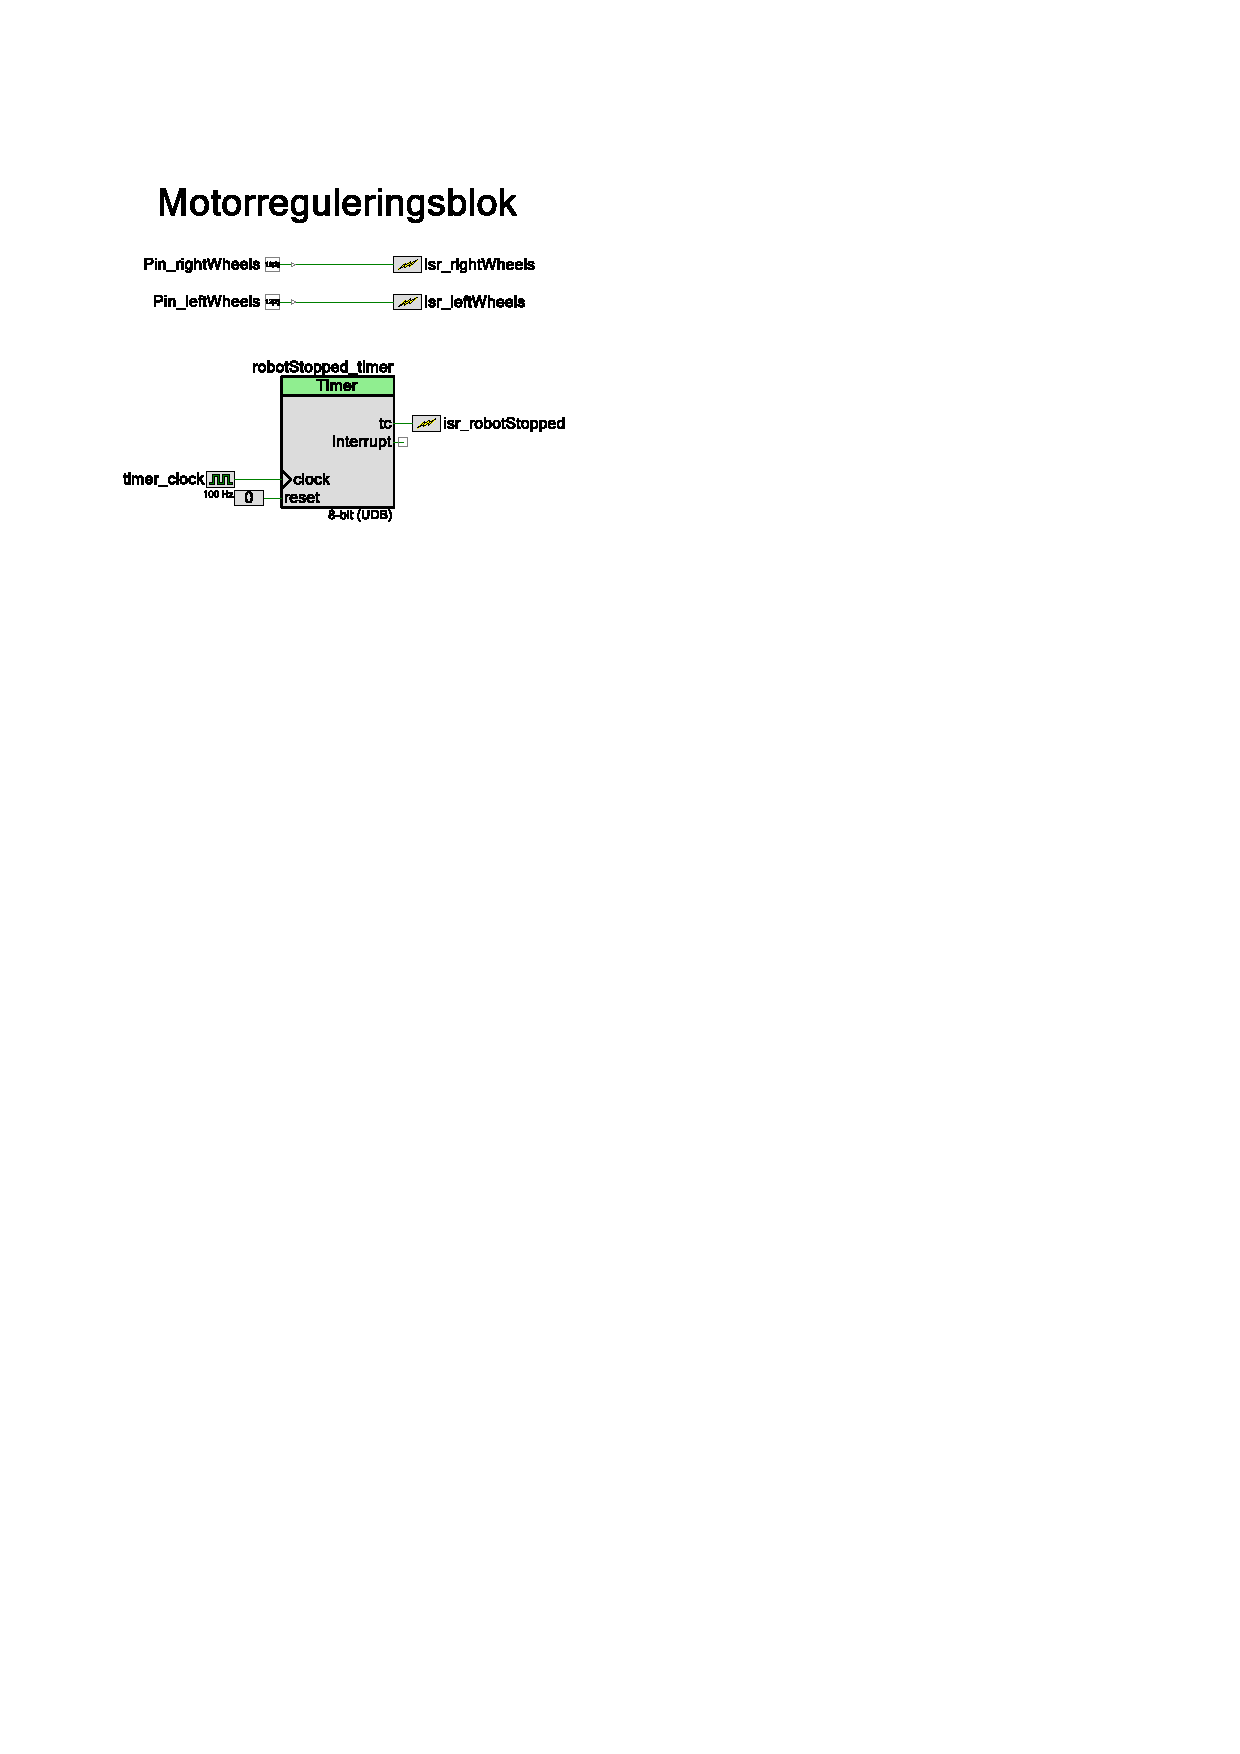
\includegraphics[clip, trim = 2cm 20.5cm 11cm 4cm , width = 0.7\textwidth]{top_regulering.pdf}
\caption{Topdesign af omdrejningssensorer, fra PSoC Creator}
\label{fig:top_regulering}
\end{figure}
Når der kommer et interrupt fra venstre hjul - kaldet \textit{isr\_leftWheels} -  tælles variablen \textit{currentSpeed} én op, og når der kommer et interrupt fra højre hjul - kaldet \textit{isr\_rightWheels} - tælles variablen én ned.
Dette resulterer i, at \textit{currentSpeed} indeholder en værdi for, hvilken hastighed det højre hjul skal have for, at det kører lige så hurtigt som det venstre; Hvis hjulene er lige hurtige, så indeholder \textit{currentSpeed} værdien \textit{startSpeed}. \\
Til at justere hastigheden, bruges funktionen \textit{speedAdjust()}. 
Denne funktion ændrer duty-cyclen af PWM-signalet, der styrer de højre hjul, med værdien af \textit{currentSpeed}, således at hjulene kommer tættere på at have samme hastighed.

Reguleringen har også til ansvar at holde styr på om robotten er i bevægelse eller om den er stoppet. Dette er implementeret med timeren, der ses på topdesignet på figur \ref{fig:top_regulering}.
Ved hvert \textit{isr\_leftWheels} interrupt, sættes \textit{robotState} til \textit{robot\_moving}. 
Hvis dette interrupt udebliver i et halvt sekund vil \textit{robotStopped\_timer} sætte \textit{robotState} til \textit{robot\_stopped}. 
Altså nulstilles \textit{robotStopped\_timer} ved hvert tandhjuls interrupt.


\subsubsection{Enhedstest}
For at teste at reguleringen virker som ønsket, laves der en test, hvor der med oscilloskop måles på tandhjulenes frekvens med og uden regulering. Testen laves efter hjulene har kørt fremad i 10 sekunder, for at garantere, at hastigheden er stabil. \\
Testen er bestået, hvis reguleringen reducerer forskellen mellem frekvenserne. \\
Testen kan findes i bilag \ref{appendix:BilagPSoCEnhedstests}.

Efter at have udført testen kan det konkluderes, at reguleringen virker som ønsket.
\\Hjulene på bilen er dog så skæve, at reguleringen alene ikke kan få bilen til at køre helt lige.


\subsection{I2C}
I2C blokken har til ansvar at sende og modtage beskeder fra kontrolenheden. Topdesignet til I2C-blokken kan ses på figur \ref{fig:top_i2c}.
\begin{figure}[H]  %BILLEDE AF TOPDESIGN!!!
\centering
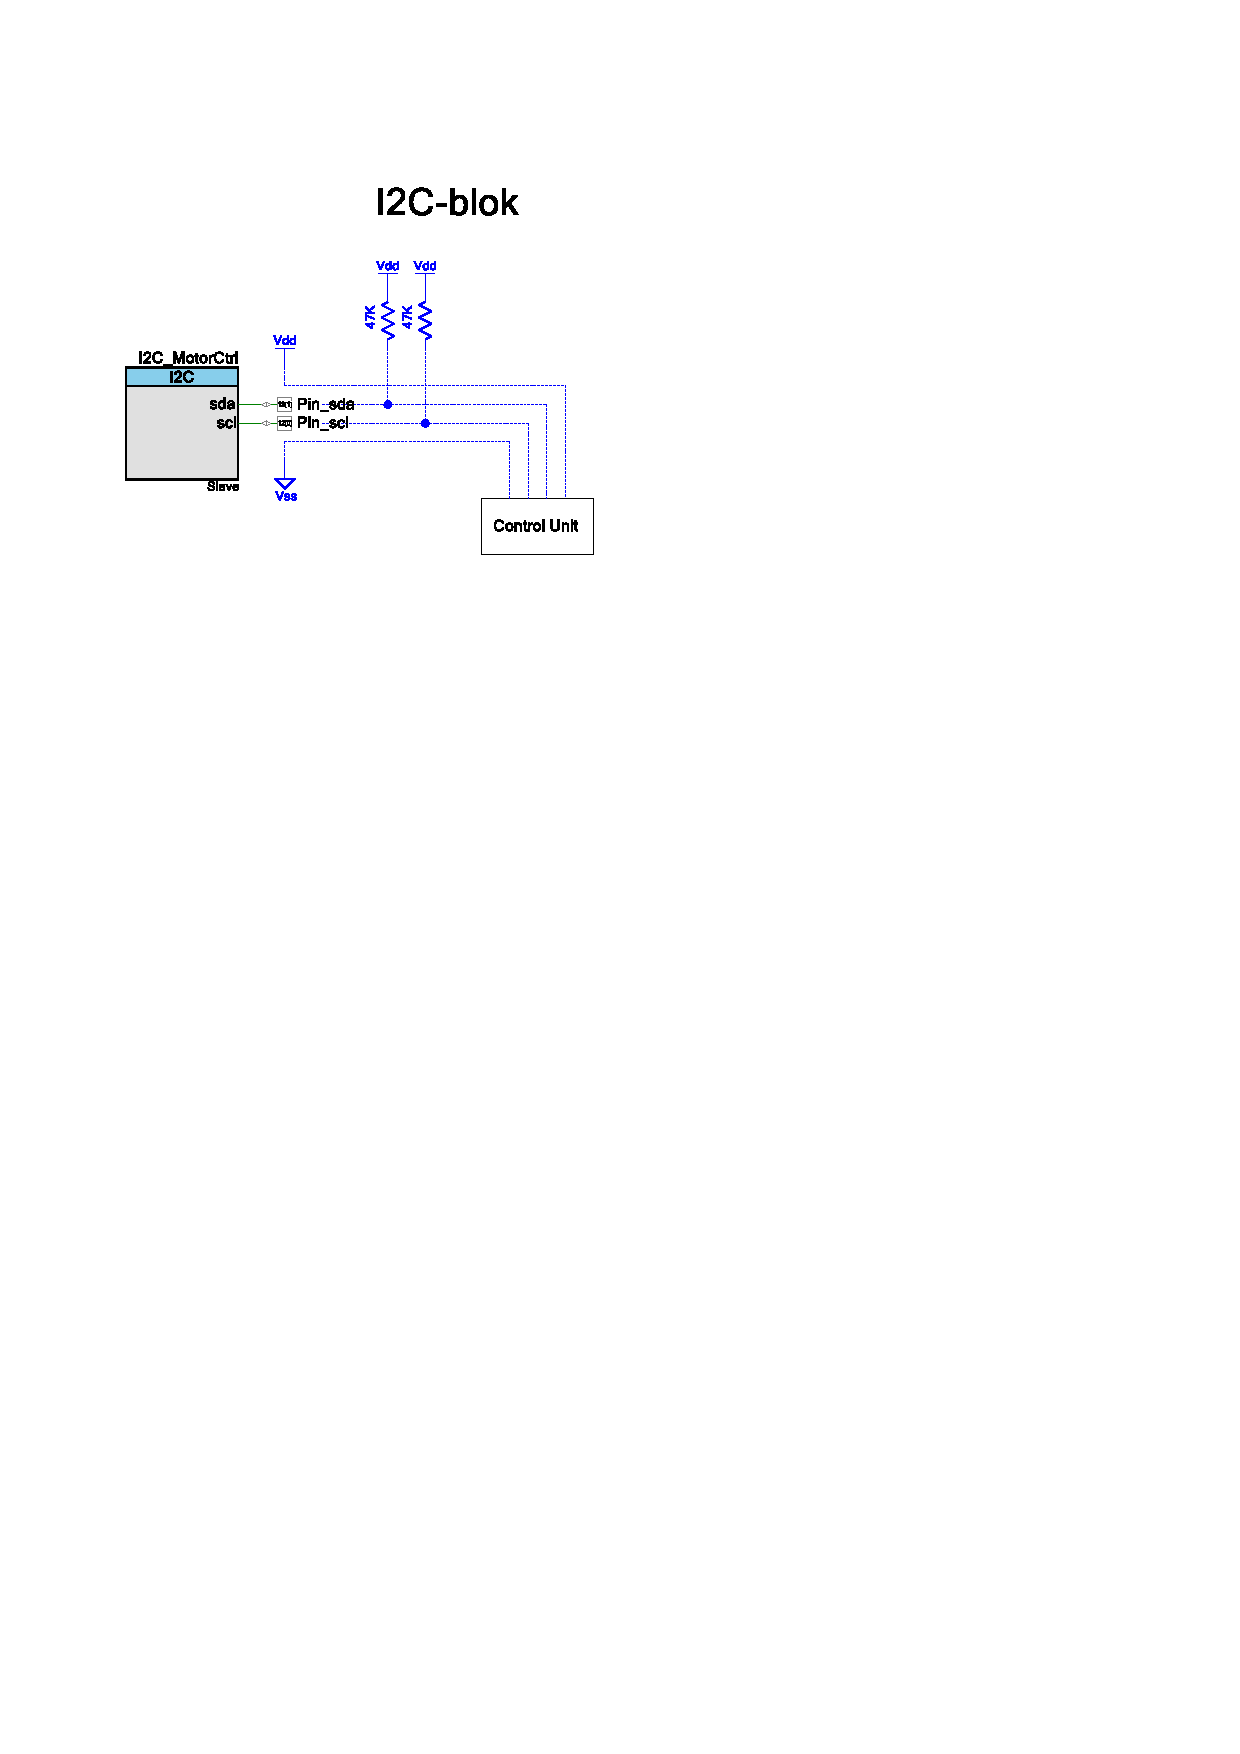
\includegraphics[clip, trim = 2cm 20cm 10cm 4cm , width = 0.7\textwidth]{top_i2c.pdf}
\caption{Topdesign af I2C, fra PSoC Creator}
\label{fig:top_i2c}
\end{figure}
De pins på PSoC'en, som bruges til I2C-forbindelsen sættes til typen \textit{open drain, drives low}, hvilket betyder, at der skal sættes eksterne pull-up resistorer på linjen. 

Da Pi'en benytter TTL logik, til at kommunikere med, skal I2C-linjen trækkes op til $3.3 V$. 
Denne spænding forsynes af Pi'ens GPIO-pins. 
PSoC'en bruger som udgangspunkt CMOS logic, så for at gøre det muligt at kommunikere med Pi'en, så laves det om således, at PSoC'ens pins ligeledes benytter TTL logik.

På PSoC'en er I2C blokken sat op til udelukkende at udføre slave funktionalitet, hvilket betyder at den kun kan sende beskeder, når masteren beder den om det. 
I2C funktionaliteten er implementeret i to interrupts som PSoC'en selv opretter - et til at modtage og et til at sende.\\
Modtagne beskeder indsættes af det ene interrupt ind i bufferen \textit{Writebuffer}, der initialiseres i I2CStart() funktionen. 
Beskeder der skal sendes indsættes i bufferen \textit{Readbuffer}.
Indholdet af Readbuffer sendes til Kontrolenheden, når denne læser fra PSoC'en.

I2C-blokken har også til ansvar at lægge PSoC'en til at sove, når kontrolenheden sender \textit{sleep} beskeden til den. 
PSoC'ens sleep funktionalitet består i, at den stopper CPU'en, så strømforbruget reduceres. 
Dette er implementeret for at kunne opfylde kravet om, at robotten skal kunne tilgå dvaletilstand. \\
Når PSoC'en sover, er den sat til at vågne, når den modtager en matchende addresse fra Kontrolenheden. 
Dette kan lade sig gøre ved at sætte addresse sammenligningen til at ske ved brug af PSoC'ens hardwarekomponenter i stedet for software. 
På denne måde kan PSoC'en forblive i sleep mode, indtil Kontrolenheden sender startbeskeden.

\subsubsection{Integrationstest mellem PSoC og kontrolenheds I2C-klasser}
For at teste I2C-forbindelsen laves en test, hvor der sendes beskeder mellem PSoC og kontrolenhed.
Testen er gennemført, hvis det er muligt at sende og modtage beskeder mellem de to enheder. 
Testen kan ses på bilag \ref{appendix:BilagPSoCEnhedstests}.

Efter at have udført testen kan det konkluderes, at I2C kommunikationslinjen virker som ønsket.

\subsection{Main}
PSoC'ens main funktion er beskrevet på flowchart, der ses på figur \ref{fig:STM_MotorControlUnit_main}. 
\begin{figure}[H]  %BILLEDE AF TEST!!!
\centering
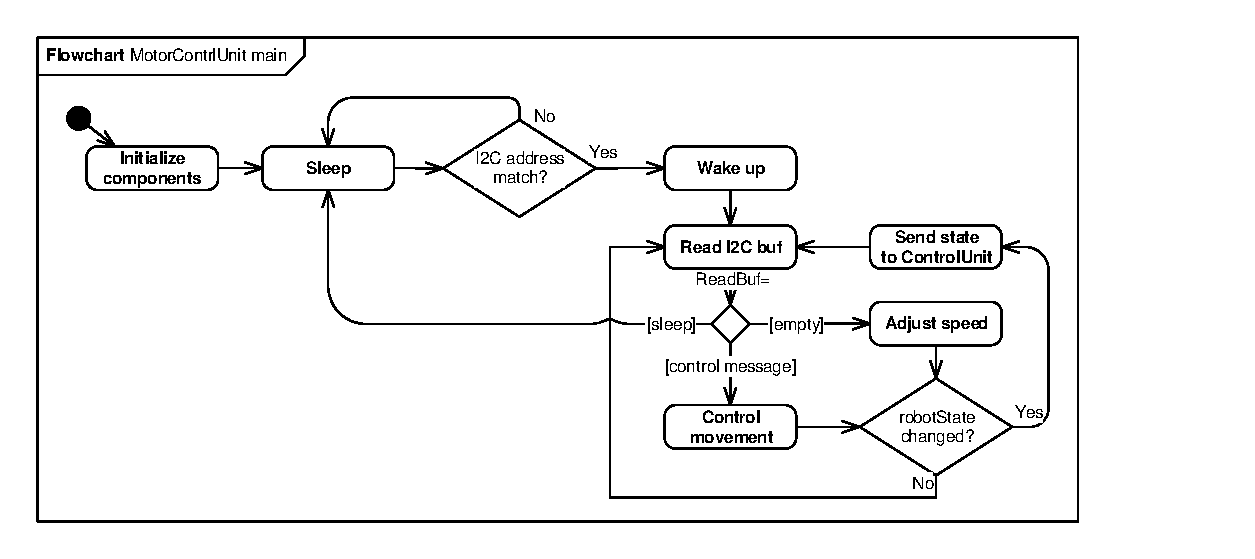
\includegraphics[clip, trim = 0.5cm 0.5cm 2.5cm 0.5cm , width = \textwidth]{STM_MotorControlUnit_main.pdf}
\caption{Tilstandsdiagram over main-funktionaliteten på Motorkontrolenheden}
\label{fig:STM_MotorControlUnit_main}
\end{figure}

Som det ses af diagrammet foretages der ikke regulering, hvis der er modtaget en kontrolbesked. 

Dette er valgt, fordi hjulene skal have tid til at køre i den ønskede retning før der reguleres.


%\end{document}